\chapter{Spacecraft Data}

	\section{\texttt{Arase}: Download and read Arase data}

	\subsection{Installation}

	Install from PyPI:
	
	\begin{minted}{bash}
	pip3 install Arase --user
	\end{minted}
	
	or
	
	\begin{minted}{bash}
	python3 -m pip install Arase --user
	\end{minted}
	
	Set the \texttt{ARASE\_PATH} variable by placing the following at the end of \texttt{\textasciitilde{}/.bashrc}:
	
	\begin{minted}{bash}
	export ARASE_PATH=/path/to/arase/data
	\end{minted}
	
	\subsection{Downloading Data}
	
	Most instrument data can be downloaded using the \texttt{DownloadData} function contained in the instruments submodule, e.g.:
	
	\begin{minted}{python}
	Arase.XXX.DownloadData(L, prod, Date=Date, Overwrite=Overwrite)
	\end{minted}
	
	where \texttt{XXX} can be replaced with the instrument names: \texttt{HEP}, \texttt{LEPe}, \texttt{LEPi}, \texttt{MEPe}, \texttt{MEPi}, \texttt{MGF} or \texttt{XEP}. \texttt{L} is an integer and \texttt{prod} is a string which correspond to the level and data product provided by the instrument, respectively (see the table in "Current Progress"). \texttt{Date} determines the range of dates to download data for. The \texttt{Date} keyword can be a single date, a list of specific dates to download, or a 2 element list defining the start and end dates (by default \texttt{Date = [20170101, 20200101]}). \texttt{Overwrite} will force the routine to overwrite existing data.
	
	This method will work for PWE data:
	
	\begin{minted}{python}
	Arase.PWE.DownloadData(subcomp, L, prod, Date=Date, Overwrite=Overwrite)
	\end{minted}
	
	where \texttt{subcomp} is the sub-component of the instrument (see table below).
	
	To download the position data:
	
	\begin{minted}{python}
	Arase.Pos.DownloadData(prod, Date=Date, Overwrite=Overwrite)
	\end{minted}
	
	where \texttt{prod} is either \texttt{'l3'} or \texttt{'def'}. The \texttt{'def'} option is needed for position-related functions elsewhere in the \texttt{Arase} module.
	
	\subsection{Position and Tracing}
	
	\begin{enumerate}
	\item Download position data:
	\begin{minted}{python}
	Arase.Pos.DownloadData('def')
	\end{minted}
	\item Convert to a binary format (this allows for quicker reading):
	\begin{minted}{python}
	Arase.Pos.ConvertPos()
	\end{minted}
	\item Save field traces:
	\begin{minted}{python}
	Arase.Pos.SaveFieldTraces(Model=Model, StartDate=StartDate, EndDate=EndDate)
	\end{minted}
	where \texttt{Model} is either \texttt{'T89'}, \texttt{'T96'}, \texttt{'T01'} or \texttt{'TS05'} (\texttt{'T96'} by default). \texttt{StartDate} and \texttt{EndDate} are the start and end dates to perform traces for, both are integers of the format \texttt{yyymmdd}.
	\item To read the position data:
	\begin{minted}{python}
	pos = Arase.Pos.GetPos()
	\end{minted}
	\item To read the traces:
	\begin{minted}{python}
	tr = Arase.Pos.ReadFieldTraces(Date)
	\end{minted}
	\end{enumerate}
	
	\subsection{Reading Data}
	
	\subsubsection{MGF Data}
	
	\begin{minted}{python}
	data = Arase.MGF.ReadMGF(Date)
	\end{minted}
	
	This returns a \texttt{numpy.recarray} object which contains the time-series data. The \texttt{Date} argument may be a single date, a list of dates, or a 2 element \texttt{list} of dates defining the start and end date to load.
	
	\subsubsection{Particle Omni-directional Spectra}
	
	\begin{minted}{python}
	data = Arase.LEPe.ReadOmni(Date)
	\end{minted}
	
	For other instruments, replace \texttt{LEPe} with one of the following: \texttt{LEPi}, \texttt{MEPe}, \texttt{MEPi}, \texttt{HEP} or \texttt{XEP}. \texttt{data} is a dictionary which will contain dates, times, energy bins, and instances of the \texttt{Arase.Tools.PSpecCls} object. The \texttt{PSpecCls} object contains all of the spectral information stored within it and is usually identified by the dictionary key containing \texttt{'Flux'}. The \texttt{PSpecCls} object has an in-built method for plotting the spectrograms, e.g.:
	\begin{minted}{python}
	data['eFlux'].Plot()
	\end{minted}
	will plot the electron flux spectrogram from the LEPe data loaded above. To list the keys of a dictionary, use \texttt{list(data.keys())}.
	
	\subsubsection{Combined Particle Spectra}
	
	Two functions are available which will load the data for multiple instruments at the same time.
	
	For electrons:
	\begin{minted}{python}
	E = Arase.Electrons.ReadOmni(Date)
	\end{minted}
	and for ions:
	\begin{minted}{python}
	H, He, O = Arase.Ions.ReadOmni(Date)
	\end{minted}
	where \texttt{E}, \texttt{H}, \texttt{He}, and \texttt{O} are all instances of \texttt{SpecCls}.
	
	\subsubsection{Single Spectra}
	
	The \texttt{SpecCls} object has the ability to return single spectra, e.g.:
	
	\begin{minted}{python}
	import Arase
	import matplotlib.pyplot as plt
	
	# read in the electrons - this should work with any SpecCls object
	spec = Arase.Electrons.ReadOmni(Date)
	
	# for the energy bins and particle flux data
	e, dJdE, _ = spec.GetSpectrum(Date, ut)
	
	# for velocity and phase space density
	v, f, _ = spec.GetSpectrum(Date, ut, xparam='V', yparam='PSD')
	
	# or to plot
	plt.figure(figsize=(8, 4))
	ax0 = spec.PlotSpectrum(Date, ut, xparam='E', yparam='Flux', Split=True, fig=plt, maps=[2, 1, 0, 0])
	ax1 = spec.PlotSpectrum(Date, ut, xparam='V', yparam='PSD', Split=True, fig=plt, maps=[2, 1, 1, 0])
	plt.tight_layout()
	
	# for more information, read the docstrings:
	spec.GetSpectrum?
	spec.PlotSpectrum?
	\end{minted}
	
	\subsubsection{3D Particle Spectra}
	
	These data are not currently placed into an object like \texttt{PSpecCls}. For instruments which provide 3D spectra, there is a function \texttt{Read3D} which will simply read the CDF file for a given date and list all of the data and corresponding metadata into two dictionaries, e.g.:
	\begin{minted}{python}
	data, meta = Arase.LEPe.Read3D(Date)
	\end{minted}
	
	\subsubsection{Pitch Angle Distributions}
	
	For particle instruments with 3D flux data, there is a method to convert these to pitch angle distributions (PADs). The PADs are calculated using the MGF data and the elevation/azimuth angles of the instruments in GSE coordinates where provided in the level 2 \texttt{3dflux} data products. It was possible to compare this method to the angles provided by the level 3 \texttt{3dflux} product from the MEPe instrument, and almost all pitch angles were within about 1-2 degrees. \textbf{WARNING: these data should be used with caution - they may not be correct.}
	
	To store the PADs:
	\begin{minted}{python}
	import Arase
	Arase.LEPe.SavePADs(Date, na=18, Overwrite=False, DownloadMissingData=True, DeleteNewData=True, Verbose=True)
	\end{minted}
	
	The above code will bin up the 3D LEPe fluxes from a single date into \texttt{na} pitch angle bins (always in the range 0 to 180 degrees). The \texttt{Overwrite} keyword will force the overwriting of previously created PAD files. \texttt{DownloadMissingData} will download any missing \texttt{3dflux} data and MGF data. \texttt{DeleteNewData} will delete the newly downloaded \texttt{3dflux} data after creating the PAD data because some of the \texttt{3dflux} files are > 500 MB.
	
	To read PADs:
	\begin{minted}{python}
	pad = Arase.LEPe.ReadPAD(Date, SpecType, ReturnSpecObject=True)
	\end{minted}
	
	This will read the PAD spectra from a single date for a given \texttt{SpecType} (e.g. \texttt{'eFlux'} or \texttt{'H+Flux'}, depending on the instrument). The returned object will either be a \texttt{dict} containing just the data if \texttt{ReturnSpecObject=False}, or a \texttt{Arase.Tools.PSpecPADCls} object if \texttt{ReturnSpecObject=True}. The \texttt{PSpecPADCls} object allows the plotting of spectrograms, 1D spectra, and 2D spectra.
	
	For a spectrogram of a specific pitch angle bin:
	\begin{minted}{python}
	pad = Arase.MEPe.ReadPAD(20180101, 'eFlux')
	pad.PlotSpectrogram(Bin=5)
	\end{minted}
	
	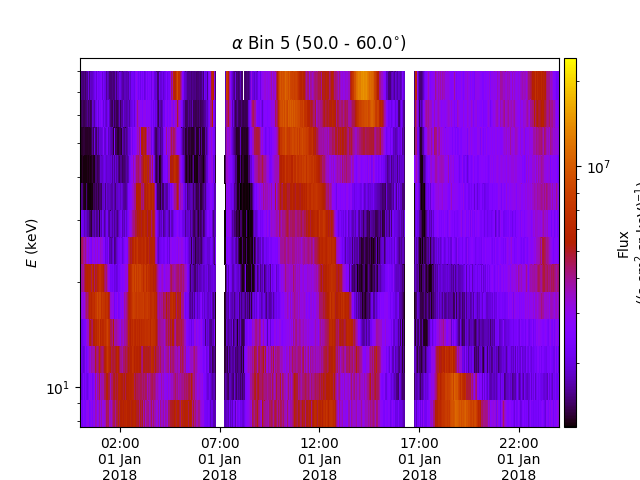
\includegraphics[width=0.8\textwidth]{figures/ch4_ArasePADSpectrogram.png}
	
	Or a 1D spectrum:
	\begin{minted}{python}
	pad.PlotSpectrum1D(12.0, Bin=5, xparam='V', yparam='PSD')
	\end{minted}
	
	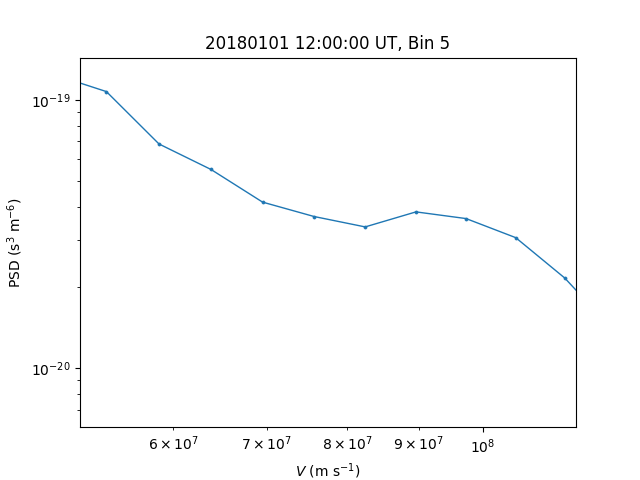
\includegraphics[width=0.8\textwidth]{figures/ch4_ArasePAD1DSpectrum.png}
	
	Or a 2D spectrum:
	\begin{minted}{python}
	pad.PlotSpectrum2D(12.0, xparam='V', zparam='PSD')
	\end{minted}
	
	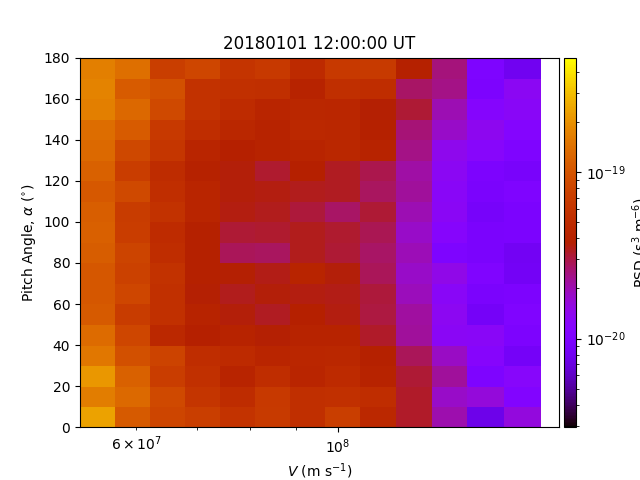
\includegraphics[width=0.8\textwidth]{figures/ch4_ArasePAD2DSpectrum.png}
	
	\subsection{Current Progress}
	
	\begin{center}
	\begin{tabular}{|l|l|l|l|l|l|l|}
	\hline
	Instrument & Subcomponent & Level & Product & Download & Read & Plot \\
	\hline
	HEP & & 2 & omniflux & \checkmark & \checkmark & \checkmark \\
	LEPe & & 2 & omniflux & \checkmark & \checkmark & \checkmark \\
	LEPe & & 2 & 3dflux & \checkmark & $\times$ & $\times$ \\
	LEPi & & 2 & omniflux & \checkmark & \checkmark & \checkmark \\
	LEPi & & 2 & 3dflux & \checkmark & $\times$ & $\times$ \\
	MEPe & & 2 & omniflux & \checkmark & \checkmark & \checkmark \\
	MEPe & & 2 & 3dflux & \checkmark & $\times$ & $\times$ \\
	MEPe & & 3 & 3dflux & \checkmark & $\times$ & $\times$ \\
	MEPi & & 2 & omniflux & \checkmark & \checkmark & \checkmark \\
	MEPi & & 2 & 3dflux & \checkmark & $\times$ & \checkmark \\
	MEPi & & 3 & 3dflux & \checkmark & \checkmark & $\times$ \\
	MGF & & 2 & 8sec & \checkmark & \checkmark & $\times$ \\
	PWE & efd & 2 & spec & \checkmark & \checkmark & \checkmark \\
	PWE & hfa & 2 & high & \checkmark & \checkmark & \checkmark \\
	PWE & hfa & 2 & low & \checkmark & \checkmark & \checkmark \\
	PWE & hfa & 3 & & \checkmark & \checkmark & $\times$ \\
	PWE & ofa & 2 & complex & $\times$ & $\times$ & $\times$ \\
	PWE & ofa & 2 & matrix & $\times$ & $\times$ & $\times$ \\
	PWE & ofa & 2 & spec & \checkmark & $\times$ & $\times$ \\
	XEP & & 2 & omniflux & \checkmark & \checkmark & \checkmark \\
	\hline
	\end{tabular}
	\end{center}
	
	\begin{itemize}
	\item \checkmark - Works
	\item $\times$ - Not working yet. In the case of 3D data, a \texttt{SpecCls3D} object needs to be written. For MGF and level 3 hfa data, it's a simple case of plotting a line.
	\item $\Diamond$ - Probably works, but have no access to the data to be able to test it.
	\item $\times\checkmark$ - Currently, 3D spectra can only be read into dictionaries as a \texttt{SpecCls3D} object is needed.
	\end{itemize}


	\section{\texttt{RBSP}: Download and read Van Allen Probe data}
	
	Some tools for loading RBSP (Van Allen Probe) data. 
	
	\subsection{Installation}
	
	Firstly, install the Python wheel package:
	\begin{minted}{python}
	pip3 install wheel --user
	\end{minted}
	
	Clone this repo, build and install (swap x.x.x for the current version):
	\begin{minted}{bash}
	git clone https://github.com/mattkjames7/RBSP.git
	cd RBSP
	
	#build the wheel
	python3 setup.py bdist_wheel
	
	#install the package just built
	pip3 install dist/RBSP-0.0.1-py3-none-any.whl --user
	\end{minted}
	
	\subsection{Submodules}
	
	This is a list of submodules contained within this package.
	
	\begin{itemize}
		\item \texttt{ECT} (see documentation in \texttt{doc/ECT.md})
		\item \texttt{EFW} (see documentation in \texttt{doc/EFW.md})
		\item \texttt{EMFISIS} (see documentation in \texttt{doc/EMFISIS.md})
		\item \texttt{Fields} (see documentation in \texttt{doc/Fields.md})
		\item \texttt{Pos} (see documentation in \texttt{doc/Pos.md})
		\item \texttt{RBSPICE} (see documentation in \texttt{doc/RBSPICE.md})
		\item \texttt{RPS} (see documentation in \texttt{doc/RPS.md})
		\item \texttt{VExB} (see documentation in \texttt{doc/VExB.md})
	\end{itemize}
	
	\subsection{ECT - Energetic Particle, Composition, and Thermal Plasma Suite}
	
	The overview of this instrument suite can be found in Spence et al., 2013.
	
	ECT contains the following instruments:
	
	\begin{itemize}
		\item Helium, Oxygen, Proton, and Electron (HOPE) Mass Spectrometer (Funsten et al., 2013)
		\item Magnetic Electron Ion Spectrometer (MagEIS, Blake et al., 2013)
		\item Relativistic Electron-Proton Telescope (REPT, Baker et al., 2013)
	\end{itemize}
	
	\subsubsection{List of Functions}
	
	The following functions are all called from within the \texttt{ECT} submodule, e.g.: \texttt{RBSP.ECT.DownloadData()}
	
	\begin{tabular}{|l|l|l|}
	\hline
	Function Name & Description & Section \\
	\hline
	\texttt{DownloadData()} & Download latest data files. & \\
	\texttt{ReadCDF()} & Read a downloaded CDF file. & \\
	\texttt{DataAvailability()} & Checks what dates have data. & \\
	\texttt{DeleteDate()} & Deletes data from a specific date. & \\
	\texttt{RebuildDataIndex()} & Scan the downloaded data and rebuild the index file. & \\
	\texttt{ReadHOPESA()} & Read the HOPE Spin-Averaged data into a \texttt{PSpecCls} object. & \\
	\texttt{ReadHOPEMoments()} & Read the HOPE moments. & \\
	\texttt{ReadHOPEOmni()} & Read the omnidirectional HOPE data into a \texttt{PSpecCls} object. & \\
	\texttt{SaveIonMoments()} & Save the cold ion moments. & \\
	\texttt{ReadIonMoments()} & Read the cold ion moments. & \\
	\texttt{MomentAvailability()} & Check what dates there are moments calculated for. & \\
	\texttt{CalculateIonMoments()} & Calculate the low energy ion moments. & \\
	\texttt{PlotMoments()} & Plot moments. & \\
	\texttt{PlotDensity()} & Plot density. & \\
	\texttt{PlotTemp()} & Plot the temperature. & \\
	\texttt{PlotMav()} & Plot the average ion mass. & \\
	\hline
	\end{tabular}
	
	\subsubsection{Downloading Data}
	
	Data from HOPE, MagEIS, and REPT can all be downloaded using the \texttt{DownloadData()} function. The \texttt{sc}, \texttt{Inst}, and \texttt{L} keywords determine which probe ('a' or 'b'), instrument, or level of data to download. To limit the time period over which to download data, set the \texttt{Date} keyword to a 2-element list containing the start and end dates in the format \texttt{yyyymmdd}.
	
	\begin{tabular}{|l|l|}
	\hline
	\texttt{Inst} & \texttt{L} \\
	\hline
	\texttt{'hope'} & \texttt{'l2.sectors'} \\
	\texttt{'hope'} & \texttt{'l2.spinaverage'} \\
	\texttt{'hope'} & \texttt{'l3.moments'} \\
	\texttt{'hope'} & \texttt{'l3.pitchangle'} \\
	\texttt{'mageis'} & \texttt{'l2'} \\
	\texttt{'mageis'} & \texttt{'l3'} \\
	\texttt{'rept'} & \texttt{'l2'} \\
	\texttt{'rept'} & \texttt{'l3'} \\
	\hline
	\end{tabular}
	
	Data is stored in \texttt{\$RBSP\_PATH/ECT/Inst/L/sc/} (e.g., \texttt{\$RBSP\_PATH/ECT/hope/l2.sectors/a/}) and the index file is named \texttt{\$RBSP\_PATH/ECT/Inst.L.sc.dat} which lists all of the downloaded files, their dates, and their versions.
	
	\subsubsection{Reading Data}
	
	All of the downloaded data can be read directly from the CDF files using \texttt{ReadCDF()}.
	
	Some HOPE-specific functions exist:
	
	\begin{minted}{python}
	#moment data from HOPE
	mom = RBSP.ECT.ReadHOPEMoments(Date,sc)
	
	#spin averaged data
	sa = RBSP.ECT.ReadHOPESA(Date,sc)
	
	#Omnidirectional data
	omni = RBSP.ECT.ReadHOPEOmni(Date,sc)
	\end{minted}
	
	\subsubsection{HOPE Moments}
	
	The moments provided by the data repository are warm plasma moments. The functions in this section make an attempt to calculate the cold ion moments.
	
	Prior to calculating the cold ion moments, we need to have downloaded all of the required HOPE Omni data, calculated all of the spacecraft potentials (see EFW), ExB drifts (see VExB), and downloaded all level 4 EMFISIS data (see EMFISIS).
	
	This function calculates all of the moments:
	
	\begin{minted}{python}
	mom = RBSP.ECT.CalculateIonMoments(Date,sc,MaxE=0.02)
	\end{minted}
	
	where \texttt{MaxE} is the maximum energy bin (keV) to include in the spectral integration (usually around 0.02 keV). The moments are calculated using the method described by Goldstein et al., 2014, Genestreti et al., 2017, and Goldstein et al., 2019.
	
	Moments are all saved to disk (\texttt{\$RBSP\_PATH/Moments/Ions/sc/}, where \texttt{sc} is either 'a' or 'b') using \texttt{SaveIonMoments()}.
	
	The moments can be read using:
	
	\begin{minted}{python}
	mom = RBSP.ECT.ReadIonMoments(Date,sc)
	\end{minted}
	
	\subsubsection{Plotting Functions}
	
	The ion moments can be plotted using \texttt{PlotDensity()}, \texttt{PlotTemp()}, and \texttt{PlotMav()}, or using \texttt{PlotMoments()} which uses all three of the former functions together.
	
	\begin{minted}{python}
	# The PlotMoments() function returns a list of axes
	axs = RBSP.ECT.PlotMoments(20140101,'a',ut=[12.0,24.0])
	\end{minted}
	
	The above code should produce the plot.
	\begin{figure}
		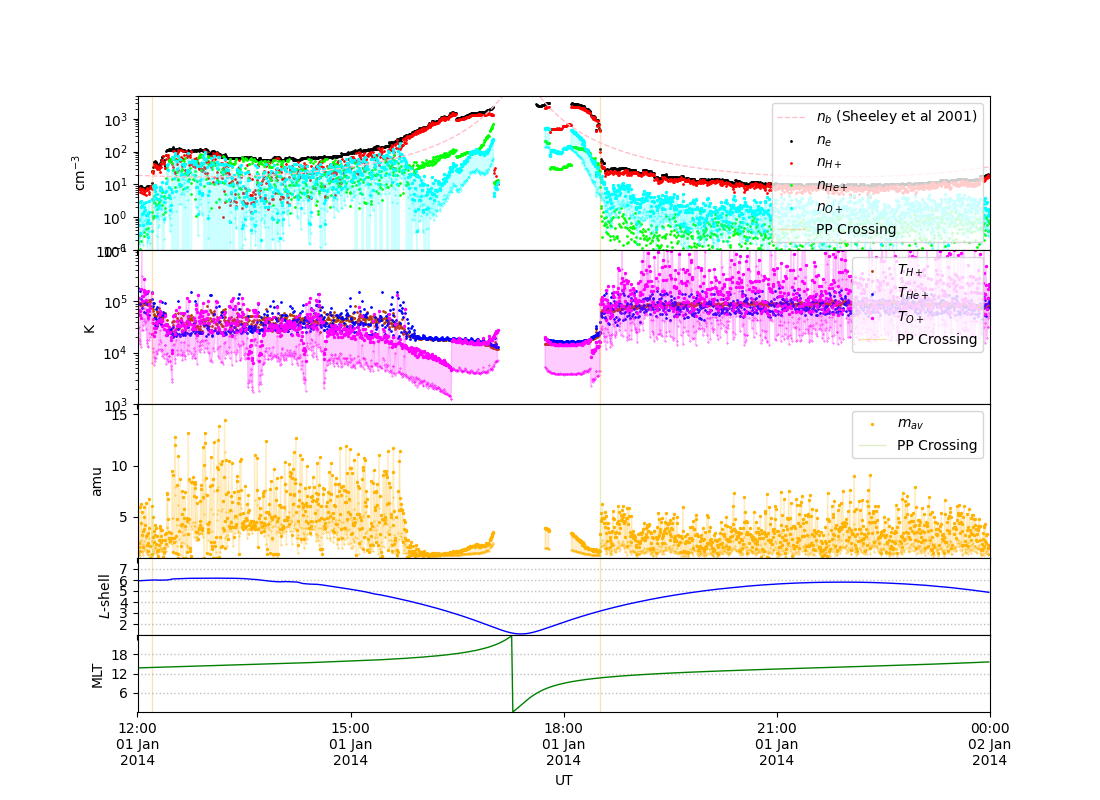
\includegraphics[width=0.9\textwidth]{figures/ch4_rbspions.png}
	\end{figure}
	
	\subsection{EFW - Electric Field and Waves}
	
	The full documentation for this instrument can be found in Wygant et al., 2013.
	
	\subsubsection{List of Functions}
	
	\begin{tabular}{|l|l|}
	\hline
	Function Name & Description \\
	\hline
	\texttt{DownloadData()} & Download latest data files. \\
	\texttt{ReadCDF()} & Read a downloaded CDF file. \\
	\texttt{DataAvailability()} & Checks what dates have data. \\
	\texttt{DeleteDate()} & Deletes data from a specific date. \\
	\texttt{RebuildDataIndex()} & Scan the downloaded data and rebuild the index file. \\
	\texttt{GetPotential()} & Get the spacecraft potential. \\
	\texttt{SavePotentials()} & Save spacecraft potentials for all dates. \\
	\texttt{ReadElectronDensity()} & Read the electron density calculated using spacecraft potential. \\
	\hline
	\end{tabular}
	
	\subsubsection{Downloading Data}
	
	The data can be downloaded using different data products, \texttt{L}:
	
	\begin{tabular}{|l|l|}
	\hline
	\texttt{L} & Description \\
	\hline
	\texttt{'l3'} & Spin-fit Electric field in modified-GSE (MGSE) coord, density, and other products \\
	\texttt{'l2.spec'} & 8 second FFT power spectra \\
	\texttt{'l2.e-spinfit-mgse'} & Spin-fit E12 Electric field in MGSE coordinates \\
	\texttt{'l2.fbk'} & 8 sample/sec filterbank peak, average wave amplitude \\
	\texttt{'l2.esvy\_despun'} & 32 sample/sec despun electric field in MGSE coordinates \\
	\texttt{'l2.vsvy-hires'} & 16 sample/sec single-ended V1-V6 probe potentials \\
	\texttt{'l1.eb1'} & EB1 in UVW coordinates \\
	\texttt{'l1.eb2'} & EB2 in UVW coordinates \\
	\texttt{'l1.mscb1'} & MSCB1 in UVW coordinates \\
	\texttt{'l1.mscb2'} & MSCB2 in UVW coordinates \\
	\texttt{'l1.vb1'} & VB1 in UVW coordinates \\
	\texttt{'l1.vb2'} & VB2 in UVW coordinates \\
	\hline
	\end{tabular}
	
	\subsubsection{Spacecraft Potentials}
	
	Spacecraft potentials need to be saved first using \texttt{SavePotentials()}, e.g.:
	
	\begin{minted}{python}
	RBSP.EFW.SavePotentials(sc)
	\end{minted}
	
	where \texttt{sc} can be 'a' or 'b'. This will save the potentials for every date found in the 'l3' data.
	
	Read the data using \texttt{GetPotential()}, e.g.:
	
	\begin{minted}{python}
	data = RBSP.EFW.GetPotential(Date,sc)
	\end{minted}
	
	\subsubsection{Electron Density}
	
	The electron densities as measured using the spacecraft potential can be obtained using the \texttt{ReadElectronDensity()} function, which is a wrapper for the \texttt{ReadCDF()} function, e.g.:
	
	\begin{minted}{python}
	data = RBSP.EFW.ReadElectronDensity(Date,sc)
	\end{minted}
	
	\subsection{EMFISIS - Electric and Magnetic Field Instrument Suite and Integrated Science}
	
	The details of this instrument can be found in Kletzing et al., 2013.
	
	\subsubsection{List of Functions}
	
	\begin{tabular}{|l|l|}
	\hline
	Function Name & Description \\
	\hline
	\texttt{DownloadData()} & Download latest data files. \\
	\texttt{ReadCDF()} & Read a downloaded CDF file. \\
	\texttt{DataAvailability()} & Checks what dates have data. \\
	\texttt{DeleteDate()} & Deletes data from a specific date. \\
	\texttt{RebuildDataIndex()} & Scan the downloaded data and rebuild the index file. \\
	\texttt{GetMag()} & Get the magnetometer data. \\
	\texttt{ReadElectronDensity()} & Get the UHR electron density. \\
	\hline
	\end{tabular}
	
	\subsubsection{Downloading Data}
	
	The data can be downloaded using different data levels and products, \texttt{L} and \texttt{Prod}:
	
	\begin{tabular}{|l|l|l|}
	\hline
	\texttt{L} & \texttt{Prod} & Description \\
	\hline
	\texttt{'l4'} & \texttt{None} & densities \\
	\texttt{'l3'} & \texttt{'1sec-***'} & 1-second resolution magnetic fields \\
	\texttt{'l3'} & \texttt{'4sec-***'} & 4-second resolution magnetic fields \\
	\texttt{'l3'} & \texttt{'hires-***'} & High-resolution magnetic fields \\
	\texttt{'l2'} & \texttt{'HFR-spectra'} & \\
	\texttt{'l2'} & \texttt{'HFR-spectra-merged'} & \\
	\texttt{'l2'} & \texttt{'HFR-spectra-burst'} & \\
	\texttt{'l2'} & \texttt{'HFR-waveform'} & \\
	\texttt{'l2'} & \texttt{'WFR-spectral-matrix'} & \\
	\texttt{'l2'} & \texttt{'WFR-spectral-matrix-burst'} & \\
	\texttt{'l2'} & \texttt{'WFR-spectral-matrix-burst-diagonal'} & \\
	\texttt{'l2'} & \texttt{'WFR-spectral-matrix-diagonal-merged'} & \\
	\texttt{'l2'} & \texttt{'WFR-spectral-matrix-diagonal'} & \\
	\texttt{'l2'} & \texttt{'WFR-waveform'} & \\
	\texttt{'l2'} & \texttt{'WFR-waveform-continuous-burst'} & \\
	\hline
	\end{tabular}
	
	Note that \texttt{***} in the above table should be replaced with the coordinate system to be used, e.g., \texttt{gsm}, \texttt{gse}, etc.
	
	\subsubsection{Mag Data}
	
	Magnetometer data can be obtained using \texttt{GetMag()} once it has been downloaded, e.g.:
	
	\begin{minted}{python}
	data = RBSP.EMFISIS.GetMag(Date,sc,ut=[ut0,ut1],Coord='GSE',Res='1sec')
	\end{minted}
	
	where \texttt{Date} may be a range or a single date; \texttt{ut} will limit the start and end times (in hours); \texttt{Coord} can be one of the following strings: 'GSE', 'GSM', 'SM', 'GEO', 'GEI'; and \texttt{Res} may be '1sec', '4sec', or 'hires'.
	
	\subsubsection{Electron Densities}
	
	Electron densities may be read from the 'l4' data using the \texttt{ReadElectronDensity()} function, e.g.:
	
	\begin{minted}{python}
	data = RBSP.EMFISIS.ReadElectronDensity(Date,sc)
	\end{minted}
	
	\subsection{Fields}
	
	This submodule combines the electric and magnetic fields.
	
	\subsubsection{List of Functions}
	
	\begin{tabular}{|l|l|}
	\hline
	Function Name & Description \\
	\hline
	\texttt{DataAvailability()} & Checks what dates have data. \\
	\texttt{CalculateEx()} & Calculates the missing E field component in MGSE. \\
	\texttt{CombineFields()} & Combines electric and magnetic field data into one object. \\
	\texttt{GetData()} & Get data for more than one date. \\
	\texttt{ModelField()} & Uses Tsyganenko field models to obtain model magnetic field vectors. \\
	\texttt{ReadData()} & Reads a single data file. \\
	\hline
	\end{tabular}
	
	\subsubsection{Usage}
	
	Get a list of dates where we have field data:
	
	\begin{minted}{python}
	dates = RBSP.Fields.DataAvailability(sc)
	\end{minted}
	
	Combine electric and magnetic fields for a single date:
	
	\begin{minted}{python}
	RBSP.Fields.CombineFields(20150101,'a')
	\end{minted}
	
	Read combined field for a date:
	
	\begin{minted}{python}
	data = RBSP.Fields.ReadData(20140503,'b')
	\end{minted}
	
	Read data between date/time limits of 20140101 12:30 to 20140103 8:15:
	
	\begin{minted}{python}
	data = RBSP.Fields.GetData([20140101,20140103],ut=[12.5,8.25],sc='a')
	\end{minted}
	
	\subsection{Pos}
	
	This submodule gets positional data for each spacecraft and can save field traces.
	
	\subsubsection{List of Functions}
	
	\begin{tabular}{|l|l|}
	\hline
	Function & Description \\
	\hline
	\texttt{CalculateVelocity()} & Calculate orbital velocity. \\
	\texttt{ConvertH5toBinary()} & Converts the downloaded position data to binary. \\
	\texttt{DownloadData()} & Downloads MagEph data. \\
	\texttt{GetPos()} & Get all position data for a spacecraft. \\
	\texttt{GetVelocity()} & Get all spacecraft velocities. \\
	\texttt{PlotL()} & Plot the $L$-shell. \\
	\texttt{PlotMLT()} & Plot magnetic local time. \\
	\texttt{ReadFieldTraces()} & Read the field line footprints for a date. \\
	\texttt{ReadAllFieldTraces()} & Read all the traces for a spacecraft. \\
	\texttt{ReadH5()} & Read the downloaded H5 data directly. \\
	\texttt{ReadPos()} & Read converted position binary data. \\
	\texttt{SaveFieldTraces()} & Saves the field line footprints. \\
	\texttt{TraceFieldDay()} & Performs field tracing for a day. \\
	\hline
	\end{tabular}
	
	\subsubsection{Usage}
	
	Download the position data first:
	
	\begin{minted}{python}
	RBSP.Pos.DownloadData(sc='a')
	\end{minted}
	
	Now convert it to binary:
	
	\begin{minted}{python}
	RBSP.Pos.ConvertH5toBinary(sc='a')
	\end{minted}
	
	Save the field line traces:
	
	\begin{minted}{python}
	RBSP.Pos.SaveFieldTraces(sc='a',Model='T96')
	\end{minted}
	
	Read in position data for the whole mission:
	
	\begin{minted}{python}
	posa = RBSP.Pos.GetPos(sc='a')
	\end{minted}
	
	Get the velocity:
	
	\begin{minted}{python}
	vela = RBSP.Pos.GetVelocity(sc='a')
	\end{minted}
	
	Get the field trace footprints:
	
	\begin{minted}{python}
	fpa = RBSP.Pos.ReadAllFieldTraces(sc='a',Model='T96')
	\end{minted}
	
	\subsection{RBSPICE - Radiation Belt Storm Probes Ion Composition Experiment}
	
	The details of this instrument can be found in Lanzerotti et al., 2013.
	
	\subsubsection{List of Functions}
	
	Not currently implemented.
	
	\subsection{RPS - Relativistic Proton Spectrometer}
	
	Details for this instrument can be found in Mazur et al., 2013.
	
	\subsubsection{List of Functions}
	
	Not currently implemented.
	
	\subsection{VExB}
	
	This submodule uses electric and magnetic fields to determine $\mathbf{E} \times \mathbf{B}$ drift, $V_{E\times B}$.
	
	\subsubsection{List of Functions}
	
	\begin{tabular}{|l|l|}
	\hline
	Function & Description \\
	\hline
	\texttt{VExB()} & Calculate drift velocity vector. \\
	\texttt{SaveData()} & Save velocity data for a single date. \\
	\texttt{ReadData()} & Read the velocity data for a single date. \\
	\hline
	\end{tabular}
	
	\subsubsection{Usage}
	
	Given arrays of electric field components \texttt{Ex}, \texttt{Ey}, and \texttt{Ez}, and magnetic field components \texttt{Bx}, \texttt{By}, and \texttt{Bz}, calculate the velocity vectors:
	
	\begin{minted}{python}
	Vx,Vy,Vz = RBSP.VExB(Ex,Ey,Ez,Bx,By,Bz)
	\end{minted}
	
	Save the field vectors for a single date:
	
	\begin{minted}{python}
	RBSP.SaveData(20170101,'a')
	\end{minted}
	
	Read those vectors back in from a file:
	
	\begin{minted}{python}
	data = RBSP.ReadData(20170101,'a')
	\end{minted}
	
	


	\section{\texttt{cluster}: Download and read Cluster data}

	Download and read in data from the Cluster mission.


	\section{\texttt{pyCRRES}: Download and read CRRES data}

	Code for the Combined Release and Radiation Effects Satellite (CRRES).


	\section{\texttt{themissc}:  Download and read THEMIS data}

	A python package to download and read THEMIS spacecraft data.

	\section{\texttt{imageeuv}: Download and read IMAGE EUV data}

	\section{\texttt{imagerpi}: Download and read IMAGE RPI data}

	\section{\texttt{imagePP}: Download and read Goldstein's plasmapause dataset}

	Simple Python code to download and use Jerry Goldstein's plasmapause database.

	\section{Installation}
	
	Clone the project and build:
	\begin{minted}{bash}
	git clone https://github.com/mattkjames7/ImagePP.git
	cd ImagePP
	
	#build the wheel file
	python3 setup.py bdist_wheel
	
	#install using pip (replace x.x.x with current version)
	pip3 install --user dist/ImagePP-x.x.x-py3-none-any.whl
	\end{minted}
	
	The \texttt{ImagePP} module requires a directory to download data to. Set the environment variable \texttt{\$PLASMAPAUSE\_DATA} prior to importing the module in Python, either in the terminal or inside \texttt{~/.bashrc}, e.g.:
	\begin{minted}{bash}
	export PLASMAPAUSE_DATA=/path/to/plasmapauses
	\end{minted}
	
	\section{Usage}
	
	On the first run, the database should be downloaded:
	\begin{minted}{python}
	import ImagePP as ipp
	
	ipp.Download()
	\end{minted}
	
	To get a specific plasmapause:
	\begin{minted}{python}
	#set date in format yyyymmdd
	Date = 20010610
	ut = 7.0
	
	#get plasmapause coordinates
	data = ipp.GetPP(Date,ut)
	\end{minted}
	
	where \texttt{data} is a \texttt{numpy.recarray} object containing plasmapause coordinates at the equatorial plane in $L$ (\texttt{data.L}) and MLT (\texttt{data.MLT}) and Cartesian $x$ (\texttt{data.x}) and $y$ (\texttt{data.y}).
	
	We can also plot that plasmapause (beware, the points are not necessarily stored in order, so results may be wild!):
	\begin{minted}{python}
	ax = ipp.PlotPP(Date,ut)
	\end{minted}
	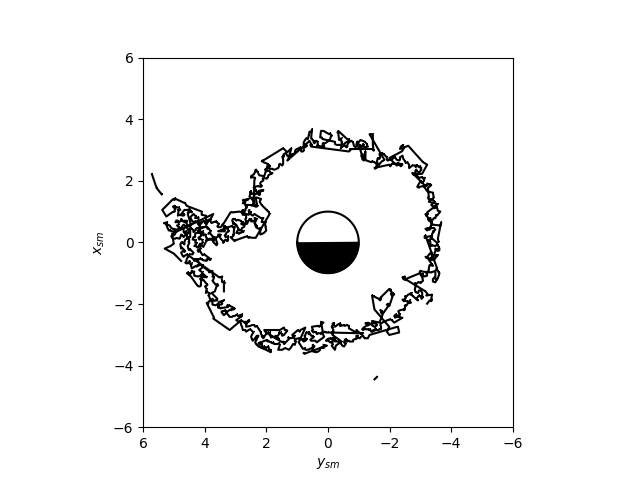
\includegraphics[width=0.5\textwidth]{figures/ch4_ppexample.png}
	

	%\section{\texttt{imagefuv}: Read IMAGE FUV data}

	\section{\texttt{PyMess}: Download and read MESSENGER data}

	A Python module for reading the MESSENGER data (or at least some of it)
	
	So far there are some tools for loading and plotting MAG, FIPS and NS data. The 
	spacecraft position can also be retrieved/plotted. A list of bow shock (BS) and
	magnetopause (MP) crossings based on the work of Winslow et al., 2013 is 
	included, which are used to provide a list of times where MESSENGER is in the 
	solar wind (SW) and the magnetosheath (MSH).
	
	In future I hope to include EPS and XRS submodules too.
	
	\subsection{Installation}
	
	Currently there is no release package on GitHub, nor is there a package 
	to PyPI, so the easiest way to install this module is to download this 
	repository, or clone it using:
	\texttt{git clone https://github.com/mattkjames7/PyMess.git}
	then to either copy the \texttt{PyMess/PyMess} subfolder to your \texttt{\$PYTHONPATH}, or 
	to create your own Python wheel:
	\begin{minted}{bash}
	cd PyMess
	python3 setup.py sdist bdist_wheel
	pip3 install dist/PyMess-0.0.1-py3-none-any.whl --user
	\end{minted}
	which may, or may not work in the code's current state!
	
	After installation, it would be wise to set up the \texttt{\$MESSENGER\_PATH}
	environment variable, as this tells the code where to find MESSENGER
	data.
	
	
	\subsection{Submodules}
	\begin{itemize}
		\item \texttt{FIPS}
		\item \texttt{MAG}
		\item \texttt{NS}
		\item \texttt{Pos}
		\item \texttt{BowShock}
		\item \texttt{Magnetopause}
		\item \texttt{Magnetosheath}
		\item \texttt{ModelField}
		\item \texttt{Tools}
	\end{itemize}
	
	\subsubsection{\texttt{FIPS} - Fast Imaging Plasma Spectrometer}
	
	This module contains routines to read FIPS plasma data. Within the \texttt{FIPS}
	submodule, there is code to convert the PDS (Planetary Data System) data
	to a more convenient format. The PDS data is stored either in ASCII or
	binary files. The ASCII files tend to be much larger than necessary, and 
	thus take a long time to read, the binary files are organised in records,
	which also take a long time to load. The following routines convert both
	types to a file format where each variable is stored contiguously within
	the file, allowing for fast reading times and smaller files.
	
	To convert to binary files, run:
	
	\begin{minted}{python}
	PyMess.FIPS.PDS.ConvertToBinary()
	\end{minted}
	
	which will scan the \texttt{\$MESSENGER\_PATH/FIPS/PDS} folder for the PDS files.
	
	Another recommended routine combines the new binary files into 1-minute 
	resolution binary files:
	
	\begin{minted}{python}
	PyMess.FIPS.Combine60sData()
	\end{minted}
	
	In future, there will be a routine to combine the high time resolution 
	data also.
	
	To load converted data, use the \texttt{PyMess.FIPS.ReadFIPS} 
	function, e.g.:
	
	\begin{minted}{python}
	data = PyMess.FIPS.ReadFIPS(Date,Type=Type)
	\end{minted}
	
	where \texttt{Date} is a 32-bit (or more) integer date in the format yyyymmdd,
	and \texttt{Type} is a string to say the type of data to load, this string can
	be one of the following:
		
		\begin{itemize}
			\item 'edr' - To load the EDR data
			\item 'cdr' - To load the CDR data
			\item 'ntp' - To load the DDR NTP data
			\item 'espec' - To load the DDR ESPEC data
			\item '60' - To load the combined 60s data (default)
			\item '10' - To load the combined 10s data
		\end{itemize}
	
	\subsubsection{\texttt{MAG} - Magnetometer}
	
	This module contains some basic routines to convert, read and plot the
	magnetometer data.
	
	To convert PDS data, download PDS data and extract data to \texttt{\$MESSENGER\_PATH/MAG/PDS}.
	Convert the PDS .TAB files using
	
	\begin{minted}{python}
	PyMess.MAG.PDS.ConvertToBinary()
	\end{minted}
	
	which should reduce the size of the dataset from GB to GB.
	
	By default, the magnetometer data used is in MSO coordinates, but we can
	also rotate the data into a coordinate system more useful for studying 
	ULF waves. In this coordinate system, there is one component parallel to 
	the ambient magnetic field; one oriented in the toroidal/azimuthal 
	direction (eastward); the third component completes the right-handed set 
	and points in the approximately poloidal/radial direction. To convert to
	these coordinates, run
	
	\begin{minted}{python}
	PyMess.MAG.SaveAllRotatedData()
	\end{minted}
	
	To read converted data, for MSO data:
	
	\begin{minted}{python}
	data = PyMess.MAG.ReadMagData(Date)
	\end{minted}
	
	For rotated data:
	
	\begin{minted}{python}
	data = PyMess.MAG.ReadRotatedData(Date)
	\end{minted}
	
	Also, for magnetopause normal data (based on the magnetopause used by
	the KT17 magnetic field model):
	
	\begin{minted}{python}
	data = PyMess.MAG.MagDataMPN(Date)
	\end{minted}
	
	To plot data:
	
	\begin{minted}{python}
	PyMess.MAG.PlotMagData(Date,ut=ut,MagType=MagType)
	\end{minted}
	
	Where, \texttt{Date} is a one or two element integer, with the format yyyymmdd,
	\texttt{ut} is a two element list, array or tuple, denoting the time range 
	(from 0 - 24)  and \texttt{MagType} is a string equal to one of the following:
	\texttt{'MSM'}|\texttt{'Rotated'}|\texttt{'MPN'}.
	
	All of the aforementioned routines have a range of keywords which can be
	found in their docstrings.
	
	\subsubsection{\texttt{NS} - Neutron Spectrometer}
	
	This submodule contains some basic routines to convert the NS PDS data 
	to a better binary format, and also to read the new data.
	
	To convert PDS data, place PDS files in \texttt{\$MESSENGER\_PATH/NS/PDS}, where the code will look
	for them, then run:
	
	\begin{minted}{python}
	PyMess.NS.PDS.ConvertToBinary()
	\end{minted}
	
	To read converted data:
	

	\section{\texttt{FIPSProtonData}: Download and read ANN verified FIPS moments}


	This Python package was written to provide a simple mechanism for 
	reading and plotting the plasma moments calculated for the MESSENGER 
	FIPS proton spectra.
	
	The moments were found by numerically fitting the kappa distribution 
	function to each proton spectrum using the downhill-simplex method. The
	quality of each fit was then assessed using neural networks, which 
	classified each spectrum as either "good" or "bad".
	
	\textbf{WARNING:} This is not yet published - do not use for anything serious yet!
	
	\subsection{Requirements}
	The following requirements should be installed automatically when using 
	\texttt{pip3} to install the package:
	
	\begin{itemize}
		\item Python 3
		\item numpy
		\item matplotlib
		\item DateTimeTools
		\item scipy
	\end{itemize}
	
	\subsection{Installation}
	\subsubsection{For Linux and possibly Mac:}
	\begin{enumerate}
		\item Download the latest released wheel \href{https://github.com/mattkjames7/FIPSProtonData/releases/download/0.0.1/FIPSProtonData-0.0.1-py3-none-any.whl}{here}.
		\item Open terminal in folder where the wheel was downloaded to.
		\item Use \texttt{pip3} to install the wheel, e.g. 
		\begin{minted}{bash}
		pip3 install FIPSProtonData-0.0.1-py3-none-any.whl --user
		\end{minted}
		where the \texttt{--user} flag will install the package locally. Replace 
		the file name above with the name of the downloaded wheel.
	\end{enumerate}
	
	\subsubsection{Windows:}
	\begin{enumerate}
		\item In cmd type \texttt{format C:}
		\item Install Linux.
	\end{enumerate}
	
	\subsection{Usage}
	\subsubsection{First run}
	Ideally you would set up an environment variable called 
	\texttt{MESSENGER\_PATH} which points to a writable directory where you store 
	MESSENGER data, e.g. 
	\begin{minted}{bash}
	export MESSENGER_PATH=/data/path/to/MESSENGER
	\end{minted}
	This can be done in your .bashrc file, or just run it before
	starting \texttt{python3} or \texttt{ipython3}.
	
	To start using the module, open \texttt{python3} or \texttt{ipython3} and run:
	\begin{minted}{python}
	import FIPSProtonData as fpd
	\end{minted}
	As the module is imported, it will try to find the \texttt{MESSENGER\_PATH} if 
	it is set, if not it will use the current working directory.
	
	\subsubsection{Loading data}
	To read in the data simply type in something to the effect of the 
	following:
	\begin{minted}{python}
	data = fpd.GetData()
	\end{minted}
	The first time the \texttt{GetData} function is called, it will search the 
	current \texttt{MESSENGER\_PATH} for the data file, then download it when it 
	finds that the file doesn't exist. The data will be downloaded to a 
	subdirectory, \texttt{\$MESSENGER\_PATH/FIPS/}.
	
	The \texttt{data} object is a \texttt{numpy.recarray} object, containing the following
	fields:
	
	\begin{tabular}{|l|l|l|}
		\hline
		Fields & dtype & Description \\
		\hline
		Date & int32 & Date in format yyyymmdd \\
		ut & float32 & UT in format hh.hhhhh... \\
		mlatn & float32 & Magnetic latitude of MESSENGER traced to the north \\
		mlats & float32 & Magnetic latitude of MESSENGER traced to the south \\
		latn & float32 & Latitude of MESSENGER traced to the north \\
		lats & float32 & Latitude of MESSENGER traced to the south \\
		mltn & float32 & Magnetic local time of MESSENGER traced to the north \\
		mlts & float32 & Magnetic local time of MESSENGER traced to the south \\
		lctn & float32 & Local time of MESSENGER traced to the north \\
		lcts & float32 & Local time of MESSENGER traced to the south \\
		mlte & float32 & MLT of equatorial trace footprint \\
		lshell & float32 & L-shell of equatorial footprint \\
		fl\_len & float32 & Field line length in Rm \\
		x & float32 & X-msm coordinate or MESSENGER in Rm \\
		y & float32 & Y-msm coordinate or MESSENGER in Rm \\
		z & float32 & Z-msm coordinate or MESSENGER in Rm \\
		Loc & U2 & String of 'MS','MP','SH','BS','SW','UK' \\
		n & float32 & Density in cm\(^{-3}\) \\
		t & float32 & Temperature in MK \\
		K & float32 & Kappa parameter \\
		Bx & float32 & X component of local magnetic field \\
		By & float32 & Y component of local magnetic field \\
		Bz & float32 & Z component of local magnetic field \\
		Rsm & float32 & Radial distance of subsolar magnetopause in Rm \\
		Rau & float32 & Radial distance of Mercury from the Sun in AU \\
		Class & int8 & Indicator of good (==1) or bad (==0) spectrum \\
		\hline
	\end{tabular}
	
	The fields in \texttt{data} are easy to access, e.g.:
	\begin{minted}{python}
	x = data[i].lshell # single element access
	x = data.lshell[i] # single element access, equivalent to above
	x = data.lshell # array access, x becomes a numpy.ndarray
	\end{minted}
	
	The field line traces which provide the field line length, equatorial
	footprint, and planetary footprint information were traced using the KT17
	magnetic field model (Korth et al., 2015; Korth et al., 2017), the code
	for which can be found in \url{https://github.com/mattkjames7/KT17}.
	
	The \texttt{Loc} variable corresponds to the location of MESSENGER in Mercury's
	plasma environment at the time of the FIPS measurement. These locations 
	were found using the method described in Winslow et al., 2013.
	
	\subsubsection{Plotting data}
	There are two plotting routines which come with this module: 
	\texttt{fpd.PlotParameter} and \texttt{fpd.QuickPlot}.
	
	\texttt{QuickPlot} will plot *n*, *T*, \(\kappa\), \(B_x\), \(B_y\),
	\(B_z\), and \(\pm|\mathbf{B}|\) on a single page using:
	\begin{minted}{python}
	fpd.QuickPlot(Date,ut,ShowClass=True)
	\end{minted}
	where \texttt{Date} is either a single integer or a two-element list, tuple, or
	array of integers in the format *yyyymmdd*, e.g., 12th June 2014 is formatted
	20120612. \texttt{ut} is a two-element list, tuple, or array
	of floating-point values, where the time is formatted in hours, so a
	time of 13:45:00 would be written as 13.75 (i.e. hh + mm/60 + ss/3600).
	\texttt{ShowClass} is a Boolean value and shows whether each spectral fit was
	considered to be good or bad by shading the background either green or red,
	respectively.
	
	\texttt{PlotParameter} is used to plot a single parameter, where one may choose
	from 'n', 'T', 'K', 'Bx', 'By', 'Bz', 'B', or 'Class', e.g.:
	\begin{minted}{python}
	fpd.PlotParameter('n',Date,ut)
	\end{minted}
	
	\texttt{Date} and \texttt{ut} are the same format as for \texttt{QuickPlot}, all other 
	keyword arguments can be found in the docstring by typing:
	\begin{minted}{python}
	fpd.PlotParameter?
	\end{minted}
	

	\section{\texttt{VenusExpress}: Download and read VEX data}